\documentclass[a4paper]{article}
\usepackage[a4paper, margin=1.5in]{geometry}
\usepackage[utf8]{inputenc}
\usepackage[serbian]{babel}
\usepackage{graphicx}
\usepackage{url}
\usepackage{listings}

\makeatletter
\renewcommand\@biblabel[1]{\textbullet}

\title{Sistem za navigaciju baziran na OpenStreetMap-u}
\author{Nikola Bebić}
\date{Jun 2020}

\begin{document}

\begin{titlepage}
    \centering
    
\includegraphics[width=1\linewidth]{usnp.png}
    
    \vspace{8em}
    
    \@author
    
    \vspace{4em}
    
    {\bfseries\huge
        \@title
    }
    
    \vspace{2em}
    
    {\large
        Projekat iz kursa Veštačka Inteligencija
    }
    \vfill
    Novi Sad, \@date
\end{titlepage}

\makeatother

\tableofcontents

\newpage

\section{Uvod}

OpenStreetMap je besplatna, slobodna mapa celog sveta koju svi mogu da uređuju.
Podaci su dostupni pod slobodnom licencom, što dozvoljava njihovu upotrebu i primenu.
U ovom projektu korišćen je mali deo ovih podataka, koji geografski pripada užem delu Novog Sada.

Svi podaci u mapi su predstavljeni preko čvorova \emph{(Nodes)}, staza \emph{(Ways)} i relacija \emph{(Relations)}.
Čvorovi predstavljaju osnovnu jedinicu mape, i sadrže svoju geografsku dužinu i širinu.
Sami za sebe mogu predstavljati mesta od interesa, oznake objekata i slične objekte.
Staze se sastoje od niza čvorova, i mogu predstavljati kolovoze, trotoare, reke, ivice objekata, parkova, i slično. Relacije nisu korišćene u ovom projektu.

Svi objekti sadrže \emph{atribute}, odnosno niz parova ključ-vrednost koji definišu šta predstavlja neki čvor ili staza, kao i detaljnije opisuje taj objekat.
U ovom projektu od značaja je bio atribut \emph{``highway"} koji označava bilo kakav put (kolovoz, trotoar, biciklističku stazu, ...).
Vrednost tog atributa definiše tačno o kom tipu puta se radi.

U ovom projektu korišćeni su ovi podaci kao osnova za kreiranje sistema za navigaciju po gradu.
Sistem omogućava pronalaženje najkraćek, kao i najbržeg puta između neke dve tačke na mapi.

\newpage

\section{Priprema podataka}

Pri pokretanju programa podaci o mapi se učitavaju iz fajla. Već prilikom učitavanja kreiraju se sledeće strukture:

\begin{itemize}
    \item \lstinline{node_dict} - heš-mapa koja preslikava identifikacioni broj čvora na entitet čvora. U ostatku programa se koriste samo identifikacioni brojevi čvorova, pa je ova mapa potrebna kada su potrebni i ostali atributi čvorova (pre svega geografska dužina i širina)
    \item \lstinline{nodes} - heš-mapa koja preslikava identifikacioni broj čvora u listu njegovih suseda, gledajući samo u smeru upteva. Ovime se predstavlja mreža puteva kao usmereni graf. Osim identifikatora susednog čcora, čuva se i entitet puta koji ih spaja.
\end{itemize}

Pri učitavanju, uzimaju se u obzir samo putevi iz tabele \ref{tab:speeds}. Svi ostali putevi, kao i čvorovi koji se isključivo na njima nalaze su ignorisani.

Osim toga, mere se i neke metrike koje se ispisuju: broj čvorova i ivica koje su uzete u obzir. Takođe se pamte i svi putevi u grafu, kako bi se kasnije iscrtali, predstavljajući mapu.

\section{Traženje najkraćeg puta}

Za traženje najkraćeg puta korišćen je A* algoritam. Ulaz u algoritam je početni čvor u grafu, koji se mora nalaziti na nekom od puteva.

Za računanje cene grana korišćena je funkcija \lstinline{distance} koja je u ovom slučaju računa običnu geografsku udaljenost. Ulaz ove funkcije su dva čvora, a izlaz cena puta između njih.

Pošto su udaljenosti male, koristi se jednostavna formula za rastojanja, koja računa rastojanja na normalnoj projekciji Zemlje.

\[
    d (a, b) = \sqrt{ ( H ( a_{lon} - b_{lon} ) ) ^ 2 + ( a_{lat} - b_{lat} ) ^ 2 }
\]
gde je $H$ konstanta čija vrednost zavisi od geografske širine. Za Novi Sad ona iznosi $ \cos 45.2551338 = 0.13402739523 $. Generalno se računa kao kosinus srednje geografske širine za tačke koje se posmatraju. \footnote{Rezultujuća vrednost e u stepenima kružnog luka. Kako bi se dobila stvarna udaljenost na površini, potrebno je sve distance pomnožiti sa $\frac{R \pi}{180}$, gde je $R$ poluprečnik Zemlje.}

Nakon računanja distance svih suseda, ukoliko je čvor već ubačen u red opsluživanja, njegov prioritet se podešava ukoliko je povoljniji od trenutnog (relaksacija), i red se ponovo \emph{heapify}-uje. Ukoliko nije već ubačen, samo se ubacuje u red.

Prilikom ubacivanja (ili relaksiranja) čvora u red, pamti se njegov \emph{predhodnik} (trenutni čvor), kako bi se put na kraju mogao rekonstruisati.

Ukoliko se iz reda izvuče ciljni čvor, algoritam se zaustavlja. Rezultat se može pronaći praćenjem niza predhodnika. Ukupan put je u ovom slučaju težina ciljnog čvora.

\section{Traženje najbržeg puta}

Drugi način funkcionisanja je da se traži (očekivani) najbrži put. Ovo se može postići modifikovanjem cena na putevima, kako bi se uračunala očekivana brzina.

Jedina razlika sa predhodnim algoritmom je u funkciji distance: Ona osim čvorova sada prima i tip puta, i rezultat skalira sa preferencijom tog puta.

\[
    d(a, b, w) = d'(a, b) / w_{pref}
\]
gde je $d'$ obična distanca iyz predhodnog poglavlja, a $w_{pref}$ preferencija puta, čije se vrednosti u zavisnosti od tipa puta mogu videti u tabeli \ref{tab:speeds}.

U ovom slučaju, rezultujuća udaljenost ne predstavlja stvarnu udaljenost, te ju je potrebno izračunati naknadno, računanjem udaljenosti među pojedinačnim čvorovima.

Problemi sa trenutnom implementacijom su to što su vrednosti za preferencije puteva proizvoljne i ``odokativne''. Bolji pristup bi bio da te preferencije uzimaju u obzir prosečne brzine vozila na tim deonicama. Takođe ne uzimaju se u obzir vremena provedena ``na čvorovima'', odnosno vremena čekanja na raskrsnicama, vreme potrebno za skretanje, ...

\section{Korisnični interfejs}

Malo pažnje je posvećeno korisničkom interfejsu. Ulaz za 2 tačke se uzima klikom na mapu (nakon svakog klika je potrebno mapu ručno zatvoriti), nakon čega se računa rezultujući najkraći i najbrži putevi. Na kraju, najbrži i najkraći putevi se prikazuju na mapi.

Takođe, moguće je pustiti program da automatski pronalazi lokacije gde je najkraći put mnogo kraći od najbržeg. Primer jednog takvog puta dat je na slici \ref{fig:shortest_fastest}.

\begin{figure}
    \centering
    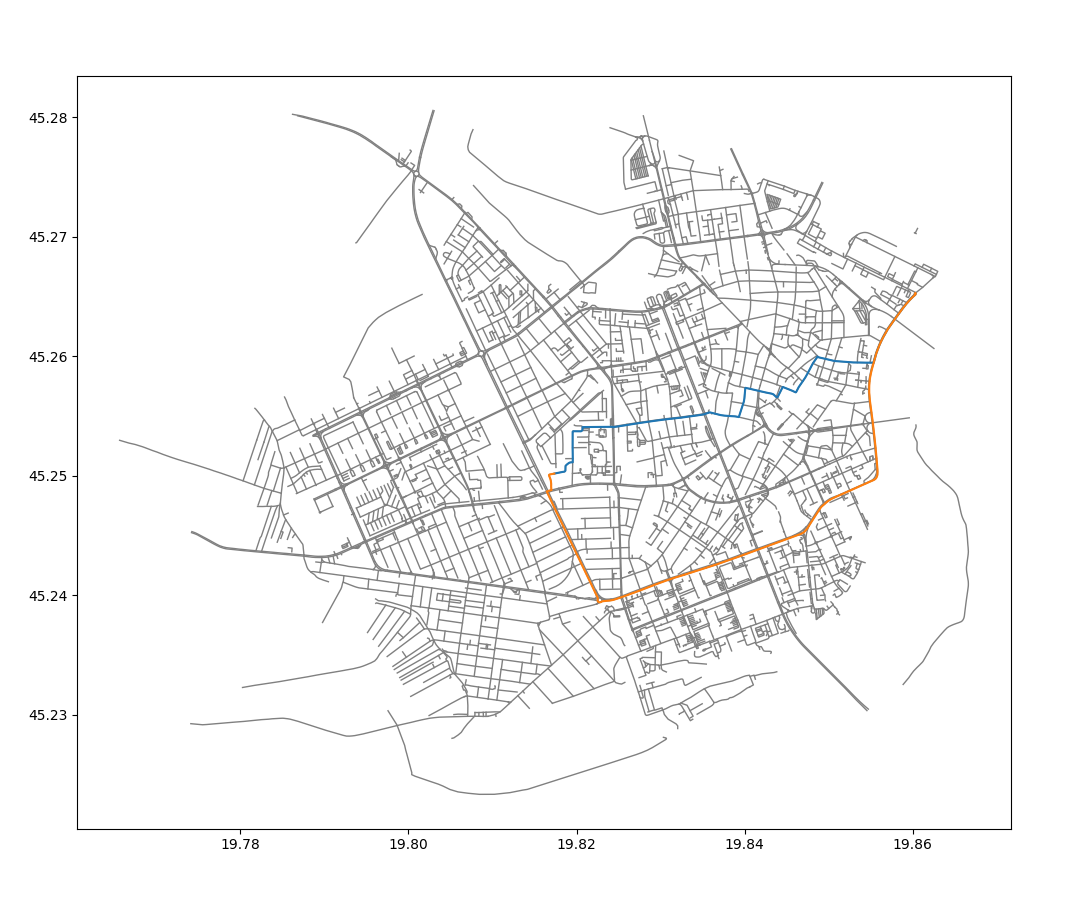
\includegraphics[width=\linewidth]{najkracem_je_najduzi.png}
    \caption{Primer gde je najkraći put (plavo) mnogo kraći od najbržeg (narandžasto). Primer od Ledinačke do Bajči Žilinskog}
    \label{fig:shortest_fastest}
\end{figure}

\section{Dodatak}

\begin{table}[h]
    \centering
    \begin{tabular}{c|c}
        `highway' vrednost & preferencija \\
        \hline
        motorway & 10 \\
        trunk & 10 \\
        primary & 10 \\
        secondary & 9 \\
        tertiary & 8 \\
        unclassified & 7 \\
        residential & 6 \\
        service & 5 \\
        motorway\_link & 9 \\
        trunk\_link & 8 \\
        primary\_link & 7 \\
        secondary\_link & 6 \\
        tertiary\_link & 5 \\
        living\_street & 4
    \end{tabular}
    \caption{Tipovi puteva uzimani u obzir, kao i njihove težinske preferencije pri računanju najbržeg puta.}
    \label{tab:speeds}
\end{table}

\end{document}
